\chapter{Parametrization of fluctuation power spectra} \label{ch:Parametrization}
\graphicspath{{chapter4_ys/}}
\minitoc


A key ingredient of our systematic study of plasma turbulence properties from fixed-frequency reflectometry power spectra, is the spectrum parametrization method. The method was developed in the course of this work and is the subject of the present chapter. The motivation for parameter reduction is given in section \ref{sec:parameter_reduction}. Section \ref{sec:spectra_fit} discusses several aspects of the spectrum fitting method, viz. the spectrum normalization, the cost function and the parametric model. Section \ref{sec:parametrization_process} provides the details of the fitting process, including boundary conditions for the parameters and global optimization. Some parametrization results and comparisons between different models are discussed in section \ref{sec:parametrization_results_and_discussion}. Finally, the parametrization method is applied to the Tore Supra database and a new turbulence database is built, as described in section \ref{sec:turbulence_database}.


\section{Parameter reduction} \label{sec:parameter_reduction}

Although manually investigating individual spectra by quantifying their properties (e.g. contribution, width and shape of different components) on a case-by-case basis is possible, systematic and standardized investigation of numerous spectra with complicated shapes requires automated methods. One of the key elements in this approach is a suitable representation of the spectra, which ideally should be interpretable in terms of the various components known to contribute to a reflectometer spectrum, in turn related to the underlying physics of plasma fluctuations. Considering the great variety of spectrum shapes (figure \ref{fig:Spectra}), acquired under widely varying plasma conditions, this is a rather ambitious goal. As described below, there are various criteria that a good spectrum representation should fulfill, but one of the most important is that it should be concise, i.e. using a limited set of parameters. Not only does this provide the best guarantee for maintaining physical interpretability, but it is also essential for the main goal of this work, i.e. to detect patterns in the spectra throughout a large database. Again with a view to physical interpretation, the best chance to detect important clusters or trends in the database is by relying on a succinct parametrization.

There are many ways to represent the frequency spectra (each spectrum has 1000 values) by fewer parameters. We decided on an approach wherein the spectrum is decomposed in several components, with every component characterized by only a few parameters. Although spectrum fitting techniques have been widely used in many research fields, such as chemical material analysis \cite{Yamashita_2008_ASS}, biology sample analysis \cite{Lieber_2003_AS}, or spectroscopic applications in fusion plasmas \cite{Nocente_2013_IEEE}, the situation in turbulence study is different. Indeed, while in regular spectrum fitting for routine applications the possible contributions to the spectrum are usually known beforehand, the composition of reflectometry spectra is much less clear. The occurrence of significant noise and unavoidable outliers further complicates the situation.


\section{Spectrum fitting} \label{sec:spectra_fit}


\subsection{Fitting criteria}

While the total number of parameters describing the spectra, $K$ should be limited for systematic studies and also to avoid overfitting, we still wish to cover all spectrum shapes observed in the database. Hence a moderate $K$ should be aimed for. Further criteria for evaluating the fit quality are:%
%%%%%%%%%%%%%%%%%%%%
\begin{itemize}

  \item \emph{flexibility}: Flexibility refers to the ability of the model to represent many different spectral shapes, as seen in figure \ref{fig:Spectra}.

  \item \emph{discrimination}: Discrimination is related to the distinguishing power of the model parameters w.r.t. the different spectral shapes, in the sense that the parameters should have moderate sensitivity to the spectral shape. Concretely, low sensitivity generates the same parameter results for all the cases, while high sensitivity leads to unstable parameters.

  \item \emph{robustness}: Robustness means that the parameters should have minimal dependence on small model deviations that are of little interest to the analysis, such as noise.

\end{itemize}


\subsection{Normalization and cost function} \label{sec:normalization_and_cost_function}

From figure \ref{fig:Spectra} it is clear that the power of the reflected signal can vary significantly (several orders of magnitude) from one spectrum to another, which can be attributed to multiple reasons. Specifically, the launched microwave power and the wire conversion losses change with wave frequency and the reflected microwave power decreases with deeper penetration. However, the absolute value of each parametric spectrum component should be comparable across spectra to allow systematic investigations. Therefore, \emph{normalization} of the power spectrum is required and here the spectrum $S(f)$ is normalized to the total integrated power of the spectrum:%
%%%%%%%%%%%%%%%%%%%%
\begin{equation}
\hat{S}(f) = \frac{S(f)}{\int_{f_{min}}^{f_{max}} S(f)\,\mathrm{d} f}.
\label{eq:Snorm}
\end{equation}
%%%%%%%%%%%%%%%%%%%%
\noindent Here, $f_{min}$ and $f_{max}$ denote the minimum and maximum frequency in the spectrum, which here we fix at $f_{min}=-500$ kHz and $f_{max}=500$ kHz (because of the 1 MHz acquisition rate). As a result, the normalized spectrum integrates to unity, allowing spectra to be compared conveniently. For simplicity, in the remainder of this thesis, the normalized spectrum is also denoted by $S(f)$. All spectra used in this study were normalized in this way before parametrization as well as the subsequent detailed analysis.


\begin{figure}[h]
\begin{centering}
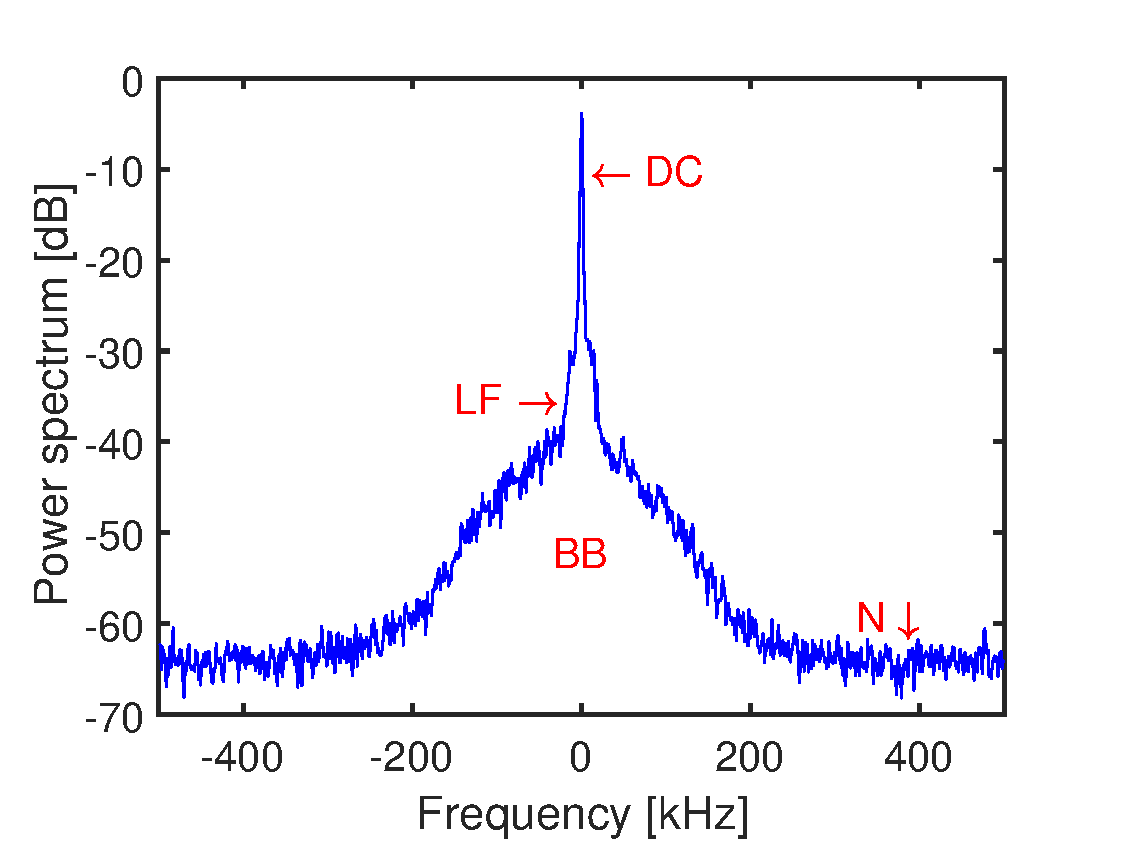
\includegraphics[scale=0.5]{fig_Spectrum.eps}
\par\end{centering}
\caption{One typical normalized spectrum (figure \ref{fig:Spectra} (a)) with the various components to be fitted. The spectrum has been normalized to its total power.}
\label{fig:Spectrum}
\end{figure}

Figure \ref{fig:Spectrum} shows a typical normalized spectrum (corresponding to figure \ref{fig:Spectra} (a)), with the various components indicated. When fitting a spectrum by minimization of the residual sum of squares (RSS), it is important to consider the scale at which to perform the fit. Generally, the logarithmic scale gives more weight to low amplitudes while the linear scale gives more weight to high amplitudes. Specifically for the spectra analyzed here, low amplitudes are usually found at high frequencies and vice verse. For this reason a combination of fitting on both the logarithmic and linear scales is performed, by minimizing the following cost function:%
%%%%%%%%%%%%%%%%%%%%
\begin{equation}
F_{cost}=(1-w)\times\frac{|\lg(S_{fit})-\lg(S)|^{2}}{A_{lg}} + w\times|S_{fit}-S|^{2}.
\label{eq:Fcost}
\end{equation}
%%%%%%%%%%%%%%%%%%%%
\noindent Here, $S_{fit} = S_{fit}(f)$ and $S = S(f)$ denote the fitting model and the normalized frequency spectrum, respectively. In addition, $A_{lg} = \int_{Fmin}^{Fmax} (lg(S))^2\,\ud f$, where $lg = 10 \times log10$, is the integral of the spectrum on the logarithmic scale, ensuring normalization of the logarithmic part of the cost function. As a result, it is possible to weigh the two parts of the cost function using a weight factor $w$, allowing a more proper fit of both the high-frequency and low-frequency parts of $S(f)$. 

In this study, we have chosen to give equal weight to the linear and logarithmic parts ($w = 0.5$) after comparing different values with some representative spectra. Experimentation with other values ($0.25$ and $0.75$) has pointed out that the results are not very sensitive to the weight factor. This does not exclude a more optimal weight factor for different spectrum decompositions or different databases. In fact, the changeable weight of the cost function has the advantage of flexibility when comparing to some other methods to realize the optimisation like the Kullback�CLeibler divergence. 


\subsection{Spectrum decomposition} \label{sec:models_of_spectra_fit}

In previous work \cite{Kramer-Flecken_2004_NF,Vershkov_2005_NF,Shelukhin_2006_PPR,Vershkov_2011_NF,Kramer-Flecken_2015_NJP}, several components were distinguished in fluctuation spectra associated to specific physical phenomena: the direct current (DC) component \cite{Kramer-Flecken_2015_NJP}, the low-frequency (LF) fluctuations \cite{Vershkov_2011_NF}, the broadband (BB) fluctuations and in some cases the quasi-coherent (QC) oscillations \cite{Shelukhin_2006_PPR}. The BB fluctuations, which cover the whole frequency range, have a short correlation length \cite{Kramer-Flecken_2015_NJP,Vershkov_2011_NF} and have been attributed to turbulence, to be called BB turbulence \cite{Vershkov_2005_NF} hereafter. Both the LF and QC components are superimposed on the BB turbulence. The LF component represents the more intense fluctuations at low frequencies. Zonal flows and certain MHD modes like sawteeth and fishbones may contribute to this component. However, at this stage, it is still difficult the exact origination of the LF component. Due to the narrow bandwidth, it is also difficult to further discriminate the more refined different contributions. In addition, a very narrow central spike at zero frequency was identified as the reflectometer carrier wave, named the DC component in \cite{Kramer-Flecken_2015_NJP}. The QC oscillations can be observed in the LFS and are linked to drift wave instabilities (TEM) \cite{Arnichand_2014_NF}. In addition, the noise (N) level should be considered as another component for completeness.

The central idea of this decomposition is that, under the condition that the decomposition provides a faithful representation of the various spectrum components, and assuming that the main contribution to the density fluctuations originates from the vicinity of the cutoff layer, systematic studies of the underlying physical phenomena and their coupling should become feasible.

As mentioned before, to enable systematic studies of trends or evolution of turbulence properties, it is important to describe the spectrum components using a limited number of parameters. This is accomplished by modeling each component by a simple parameterized function, which is able to represent the shape of the component under different physical conditions. Thus, the objective is to fit the frequency spectrum by a model $S_{fit}(f)$, written as a sum of $m$ components $C_{i}(f)$ ($i=1,\ldots,m$).

Apart from the components mentioned above, various low-frequency MHD modes (e.g. sawteeth \cite{Chapman_2011_PPCF_ST_review}, fishbones \cite{Zonca_2007_NF_Efishbone,Arnichand_2016_PPCF}, tearing modes \cite{Buttery_2000_PPCF_NTM_review}) and other high-frequency fluctuations (e.g. geodesic acoustic modes \cite{Conway_2005_PPCF,Zarzoso_2018_NF_EGAM}, Alfv\'{e}n eigenmodes \cite{Heidbrink_2006_NF,Fredrickson_2018_NF,Crocker_2018_NF}) could appear under certain conditions. Since the bandwidth of these fluctuations is relatively narrow the contribution to the total power can safely be neglected, even though their amplitudes can be large in some cases. Specifically, the bandwidth of these modes is only 10 $\sim$ 100 Hz (sawteeth) or a few or tens of kHz (fishbones, tearing modes, etc), which is usually some orders less than the bandwidth of the BB component ($\sim$ 100 kHz). The fitting results are therefore not expected to be substantially influenced in the presence of such modes. On the other hand, QC oscillations can attain significant bandwidths (tens of kHz). Low-frequency and high-frequency QC modes have been observed and examples can be found in \cite{Kramer-Flecken_2004_NF,Vershkov_2005_NF,Shelukhin_2006_PPR,Vershkov_2011_NF,Arnichand_2014_NF}. However, we did not consider QC modes in the present stage, as their contribution to the power on the logarithmic scale is limited anyway.

In summary, every spectrum is decomposed into four basic components: the direct current (DC) component, the low-frequency (LF) fluctuations, the broadband (BB) turbulence and the noise (N) level, as shown in figure \ref{fig:Spectrum}. Therefore the number of components $m$ is 4 \cite{Sun_2017_IRW13}:%
%%%%%%%%%%%%%%%%%%%%
\begin{equation}
S_{fit} = C_\mathrm{DC} + C_\mathrm{LF} + C_\mathrm{BB} + C_\mathrm{N}.
\label{eq:SfitComp}
\end{equation}
%%%%%%%%%%%%%%%%%%%%


\subsection{Components of spectrum fit} \label{sec:choice_of_components}

We now go into more details for each of the main spectrum components.

\subsubsection{The noise level}

The level of noise, assumed to be frequency-independent white noise, can be described by a single constant, therefore %
%%%%%%%%%%%%%%%%%%%%
\begin{equation}
C_\mathrm{N} = \epsilon_\mathrm{N}(f).
\label{eq:CN}
\end{equation}
%%%%%%%%%%%%%%%%%%%%
\noindent The noise level is also helpful to identify trivial spectra with low signal-to-noise ratio. In this study, the signal-to-noise ratio (SNR) is defined as the ratio between the maximum value of the BB component and the noise level. \\


\subsubsection{The low-frequency components}

The low-frequency components of the spectrum include the DC and LF components. For each component, we need at least three parameters to describe the intensity, the central position and the spectral shape. Inspired by the normalization to unity of the total spectrum, we choose various probability density functions (PDFs) to model each of the components. The Gaussian (normal) PDF is the most straightforward choice, which has been used before as a model to describe the DC and LF components of coherence spectra \cite{Kramer-Flecken_2015_NJP}. In this case, the fitting functions for the DC and the LF components are:%
%%%%%%%%%%%%%%%%%%%%
\begin{equation}
C_{i} = A_{i}\exp\biggl[-\frac{1}{2}\left(\frac{f-\mu_{i}}{\sigma_{i}}\right)^2\biggr],
\label{eq:CS&LF}
\end{equation}
%%%%%%%%%%%%%%%%%%%%
\noindent where $i$ denotes $DC$ or $LF$. The amplitude $A_{i}$, the mean value $\mu_{i}$ and the standard deviation $\sigma_{i}$ describe the intensity, central position and width of the components, respectively. For more accurate fitting of the DC component, the zero frequency is placed at the center of the spectrum by using 1025 rather than 1024 frequency bins.


\subsubsection{The broadband (BB) turbulence}

During initial attempts, the Gaussian function was also considered for the BB turbulence, but it was found insufficiently flexible to model all shapes. Indeed, the shape of the broadband can be distinctly non-Gaussian, more specifically Lorentzian (also known as Cauchy distribution) or Laplacian, with a strong peak and heavy tails, especially at the HFS. A combination of several Gaussian functions were tried as well, but that often caused the LF component to fit part of the BB and moreover the BB component could not reflect the real shape of the spectrum, as shown in figure \ref{fig:Lorentzian_by_GD}. Therefore, a more flexible function was required and the following three options were explored: \emph{the generalized Gaussian \emph{(GG)} function}, \emph{the Voigt function} and \emph{the Taylor function}. The expressions of the three models are presented below and their detailed properties can be found in Appendix \ref{appA}.


\begin{figure}[h]
\begin{centering}
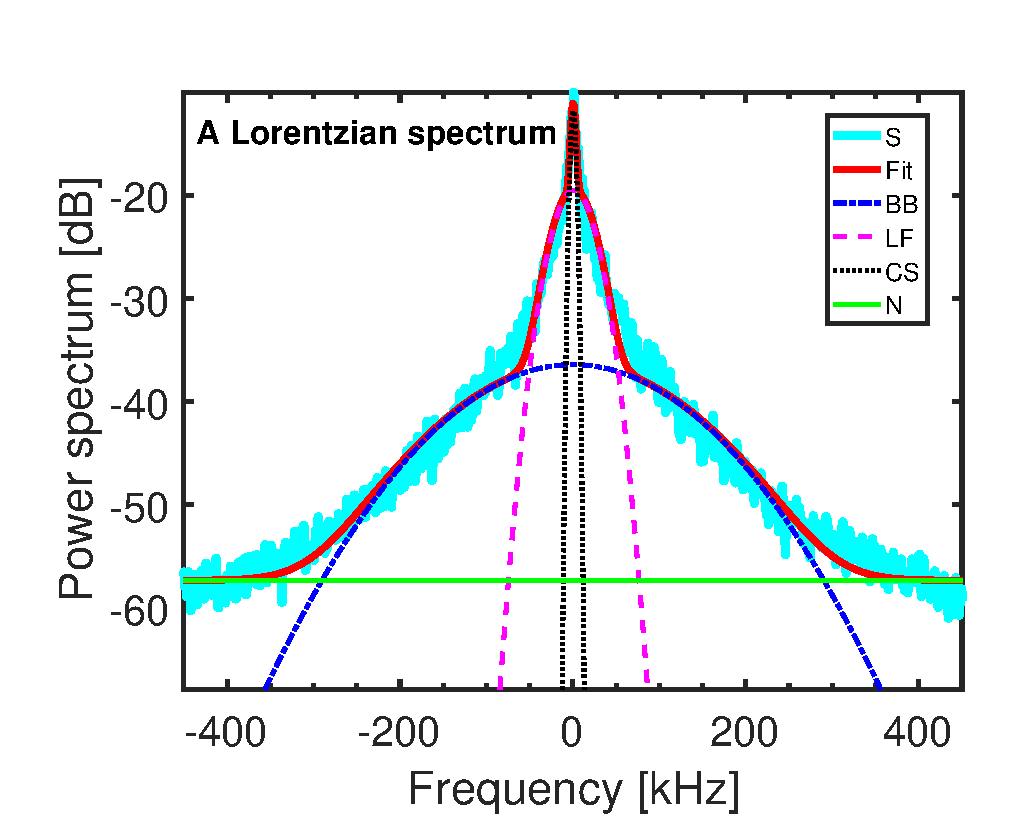
\includegraphics[scale=0.5]{fig_Lorentzian_by_GD.eps}
\par\end{centering}
\caption{A typical Lorentzian spectrum in the database fitted by multiple Gaussian functions.}
\label{fig:Lorentzian_by_GD}
\end{figure}


\paragraph*{The generalized Gaussian model}

The BB turbulence using the generalized Gaussian function becomes %
%%%%%%%%%%%%%%%%%%%%
\begin{equation}
C_\mathrm{BB}^{\textbf{GG}} = A_\mathrm{BB}\exp\biggl[-\left(\frac{|f-\mu_\mathrm{BB}|}{\alpha_\mathrm{BB}}\right)^{\beta_\mathrm{BB}}\biggr],
\label{eq:BBG}
\end{equation}
%%%%%%%%%%%%%%%%%%%%
\noindent where the fixed exponent in the Gaussian is replaced by a shape parameter $\beta_\mathrm{BB}$, and the standard deviation $\sigma_\mathrm{BB}=\sqrt{\alpha_\mathrm{BB}^2\Gamma(3/\beta_\mathrm{BB})/\Gamma(1/\beta_\mathrm{BB})}$, describing the spectral width. This function can fit multiple shapes, like Gaussian ($\beta_\mathrm{BB}=2$) and Laplacian ($\beta_\mathrm{BB}=1$).


\paragraph*{The Voigt model}

The Voigt function is a convolution of a Gaussian and a Lorentzian function:%
%%%%%%%%%%%%%%%%%%%%
\begin{equation}
C_\mathrm{BB}^{\textbf{Voigt}} =  A_\mathrm{BB}\int_{-\infty}^{+\infty} G(f;\sigma_{BBG})L(\mu_\mathrm{BB}-f;\gamma_{BBL})\,\ud f,
\label{eq:BBV}
\end{equation}
%%%%%%%%%%%%%%%%%%%%
\noindent where $G(x;\sigma)$ and $L(x;\gamma)$ are the centered (zero-mean) Gaussian and Lorentzian function, respectively, while $\mu_\mathrm{BB}$ encodes the central position of the BB component. The Voigt function has been widely used for fitting spectral lines \cite{Thompson_1987_JAC,Ida_2000_JAC}.


\paragraph*{The Taylor model}

A third alternative model for the BB component is the Taylor function. It was used in \cite{Hennequin_1999_EPS,Casati_2009_thesis} to express the correlation function of a turbulence signal in plasma physics:%
%%%%%%%%%%%%%%%%%%%%
\begin{equation}
  F_{corr}(\Delta_\mathrm{BB},\tau_\mathrm{BB}) = \exp\left[-\Delta_\mathrm{BB}(t-\tau_\mathrm{BB}+e^{-t/\tau_\mathrm{BB}})\right].
  \label{eq:Fcorr}
\end{equation}
%%%%%%%%%%%%%%%%%%%%
\noindent Here, $\Delta_\mathrm{BB}$ and $\tau_\mathrm{BB}$ are related to the wavenumber, velocity and correlation time of the turbulence, while $t$ is the sampling sequence, based on the theory of collective wave scattering by a non-uniform plasma \cite{Gresillon_1992_PPCF}. The corresponding fitting function is calculated through the Fourier transform of $F_{corr}$:%
%%%%%%%%%%%%%%%%%%%%
\begin{equation}
  C_\mathrm{BB}^{\textbf{Taylor}} = \mathrm{FFT}(F_{corr}).
  \label{eq:FFT_Fcorr}
\end{equation}
%%%%%%%%%%%%%%%%%%%%
\noindent The fitting function when considering the magnitude and the central shift can be found in Appendix A.

The number of parameters for the BB turbulence component is \emph{four}, no matter which model is used. Together with the other three components, the complete fitting model $S_{fit}$ has $K = 11$ parameters. Compared with the original 1024 (or 1025) frequency bins in the spectrum, the number of parameters has been reduced by two orders of magnitude. This parameter reduction paves the way to systematic investigations of the spectrum properties, which would have been very difficult with a large number of parameters.



\section{Fitting process} \label{sec:parametrization_process}

The spectrum fitting process is fundamentally a problem of nonlinear curve fitting or optimization. In the optimization approach, any constraints (boundary conditions) and the initial parameter values are two important factors affecting the fit.


\subsection{Constraints on component parameters} \label{sec:constraints_on_component parameters}

In order to maintain correspondence between each of the functional forms presented before and the spectrum components that they are intended to fit, additional constraints on the component parameters are necessary. To force the DC component to fit the narrow carrier wave at zero frequency, we impose the constraints $|\mu_\mathrm{DC}|<1$ kHz and $\sigma_\mathrm{DC}<2.5$ kHz, as $1$ kHz is the frequency resolution of the spectrum. For the LF fluctuations, which sometimes include high-amplitude, low-frequency MHD modes up to a few kHz, the constraints are $|\mu_\mathrm{LF}|<10$ kHz and $\sigma_\mathrm{LF}<20$ kHz. Furthermore, to avoid overlap between the DC and LF components, we require $\sigma_\mathrm{LF}>1.5\,\sigma_\mathrm{DC}$ and $\sigma_\mathrm{LF}>1$ kHz, where the factor $1.5$ was determined empirically. To summarize, the constraints on the low-frequency part are:%
%%%%%%%%%%%%%%%%%%%%
\begin{equation}
\begin{split}
& |\mu_\mathrm{DC}|<1\ \mathrm{kHz},\quad |\mu_\mathrm{LF}|<10\ \mathrm{kHz}, \\
& \sigma_\mathrm{DC}<2.5\ \mathrm{kHz},\quad 1\ \mathrm{kHz} < \sigma_\mathrm{LF}<20\ \mathrm{ kHz}, \\
& \sigma_\mathrm{LF}>1.5\,\sigma_{CS}.
\end{split}
\label{eq:ConsLF}
\end{equation}
%%%%%%%%%%%%%%%%%%%%
\noindent Constraints on the amplitudes and noise are not necessary.

For the BB turbulence, the constraints depend on the fitting functions. With the generalized Gaussian model, to separate the BB and LF components the constraints $\sigma_\mathrm{BB}>1.5\,\sigma_\mathrm{LF}$ and $\sigma_\mathrm{BB}>10$ kHz are applied, where $\sigma_\mathrm{BB}$ is the standard deviation of the BB turbulence. In addition, to avoid an overly peaked BB fit, $\beta_\mathrm{BB}$ is assumed to be larger than 0.5, the generalized Gaussian function approximating a uniform distribution for large $\beta_\mathrm{BB}$ (in practice $\beta_\mathrm{BB}>8$).

For the Voigt model, no limits have been put on the Lorentzian part. As for the Gaussian part, we use the same constraints as in the generalized Gaussian model for the standard deviation $\sigma_\mathrm{BB}$.

The parameters of the Taylor model are more difficult to constrain, as the two parameters $\Delta_\mathrm{BB}$ and $\tau_\mathrm{BB}$ jointly affect the spectral shape. Here, we set $\Delta_\mathrm{BB}>0.01$ and $\tau_\mathrm{BB}>0.01$, to avoid unrealistically peaked shapes.

The constraints for the three models are summarized as follows:%
%%%%%%%%%%%%%%%%%%%%
\begin{itemize}
  \item Generalized Gaussian model: \\ $\sigma_\mathrm{BB}>10$ kHz, $\sigma_\mathrm{BB}>1.5\,\sigma_\mathrm{LF}$, $0.5<\beta_\mathrm{BB}<8$;
  \item Voigt model: \\ $\sigma_{BBG}>10$ kHz, $\sigma_{BBG}>1.5\,\sigma_\mathrm{LF}$; %$\sigma_{BBL}<300kHz$;
  \item Taylor model: $\Delta_\mathrm{BB}>0.01$, $\tau_\mathrm{BB}>0.01$.
\end{itemize}
%%%%%%%%%%%%%%%%%%%%


\subsection{Optimization of initial conditions} \label{sec:optimization_pf_initial_conditions}

An interior-point algorithm was used for minimizing the cost function in \eqref{eq:Fcost}. A more powerful global optimizer could be employed, but this turns out to be too time-consuming in practice for a database including 350,000 spectra. Therefore, multiple starting points were chosen based on various simple criteria, increasing the chance to converge to the global minimum by simply increasing the number of initial guesses $N_{iv}$, striking a balance between computational load and goodness-of-fit.

For the DC component, $A_\mathrm{DC}$, $\mu_\mathrm{DC}$, and $\sigma_\mathrm{DC}$ were estimated by the maximum value of the spectrum, and its first and second central moments (standard deviation) in the frequency range $|f|<3$ kHz, respectively. A similar approach was taken for the LF component, but within the frequency range $3\ \mathrm{kHz}<|f|<20\ \mathrm{ kHz}$ to avoid influence by the strong DC component.

Likewise, for the BB component the parameters $A_\mathrm{BB}$ and $\mu_\mathrm{BB}$ were estimated from the maximum and the first moment of the spectrum in the frequency range $20\ \mathrm{kHz}<|f|<300\ \mathrm{kHz}$, to avoid influence of the low-frequency components. The initialization of the other parameters depends on the model.


\paragraph*{The generalized Gaussian model}


For the generalized Gaussian function, $\sigma_\mathrm{BB}$ and $\beta_\mathrm{BB}$ were estimated from the second central moment (standard deviation) and standardized fourth moment (kurtosis), respectively. Multiple initial guesses were achieved by changing the starting $\beta_\mathrm{BB}$.


\paragraph*{The Voigt model}

When fitting the BB turbulence by the Voigt function, calculation of the error function is time-consuming. The pseudo-Voigt function provides an approximation of the Voigt by using a linear combination rather than a convolution of the Gaussian and Lorentzian functions (Appendix \ref{appA}). The same constraints as for the Voigt function were used. The second central moment of the spectrum gives the initial value of $\sigma_{BBG}$ and multiple initial guesses of $\sigma_{BBL}$ were obtained by varying $\eta$.


\paragraph*{The Taylor model}

In the Taylor function, $\Delta_\mathrm{BB}$ and $\tau_\mathrm{BB}$ are slightly more difficult to estimate since they are not directly linked to the spectral shape. A tabulation of the standard deviation of $C_\mathrm{BB}^{\textbf{Taylor}}$ in \eqref{eq:Fcorr} in terms of $\Delta_\mathrm{BB}$ was made for $\tau_\mathrm{BB}=0.1$, allowing to derive initial estimates of $\Delta_\mathrm{BB}$ from the second central moment of the spectrum. Multiple initial guesses were realized by varying $\tau_\mathrm{BB}$. \\


Furthermore, to determine the number of starting points $N_{iv}$, the generalized Gaussian model is taken as an example. The initial value of $\beta_\mathrm{BB}$ estimated from the kurtosis is denoted by $\beta_{BB0}$ and was used as a first initial guess. Since $0.5<\beta_\mathrm{BB}<8$ and in the database $\beta_\mathrm{BB}$ is typically between 1 and 2, the following initial values can cover the possible spectral shapes: $\beta_{BB0}/4$, $\beta_{BB0}/2$, $2\beta_{BB0}$, $4\beta_{BB0}$. For the second initial guess, the value of $\beta_{BB0}/4$ was used, because out of all other initial values it corresponds to the shape differing the most from the shape associated with the first guess $\beta_{BB0}$ of $\beta_\mathrm{BB}$. This principle was also used to choose the third, fourth and fifth initial guess, i.e. $4\beta_{BB0}$, $\beta_{BB0}/2$ and $2\beta_{BB0}$, respectively. The convergence performance was evaluated through the averaged relative error of the overall fit for 1000 random spectra from the database, for different $N_{iv}$. From figure \ref{fig:Niv}, the relative error is near $10\%$ for a single initial value and decreases rapidly when increasing $N_{iv}$ before saturation at $N_{iv}=3$. At this point the relative error drops to $\sim1.8\%$, meaning that the results are very close to the global minimum.

For the Voigt model, $\eta=0$ and $\eta=1$ denote the Gaussian and Lorentzian shape, respectively. Therefore the first and second initial guesses were obtained by setting $\eta=0$ and $\eta=1$, followed by three more initial values in between these extremes: $\eta=0.5$, $0.25$, $0.75$. The relative fitting error saturates at around $7\%$ beyond $N_{iv}=5$. As for the Taylor model, empirical evaluation revealed a typical value of $\tau_\mathrm{BB}=0.1$. Therefore, we start from $\tau_\mathrm{BB}=0.1$ and then alternately increase and decrease according to the sequence $\tau_\mathrm{BB}=1$, $0.01$, $0.5$, $0.02$. Again, the results remain almost the same for $N_{iv}>5$, resulting in a fitting error of about $2\%$.


%%%%%%%%%%%%%%%%%%%%
\begin{figure}[h]
\begin{centering}
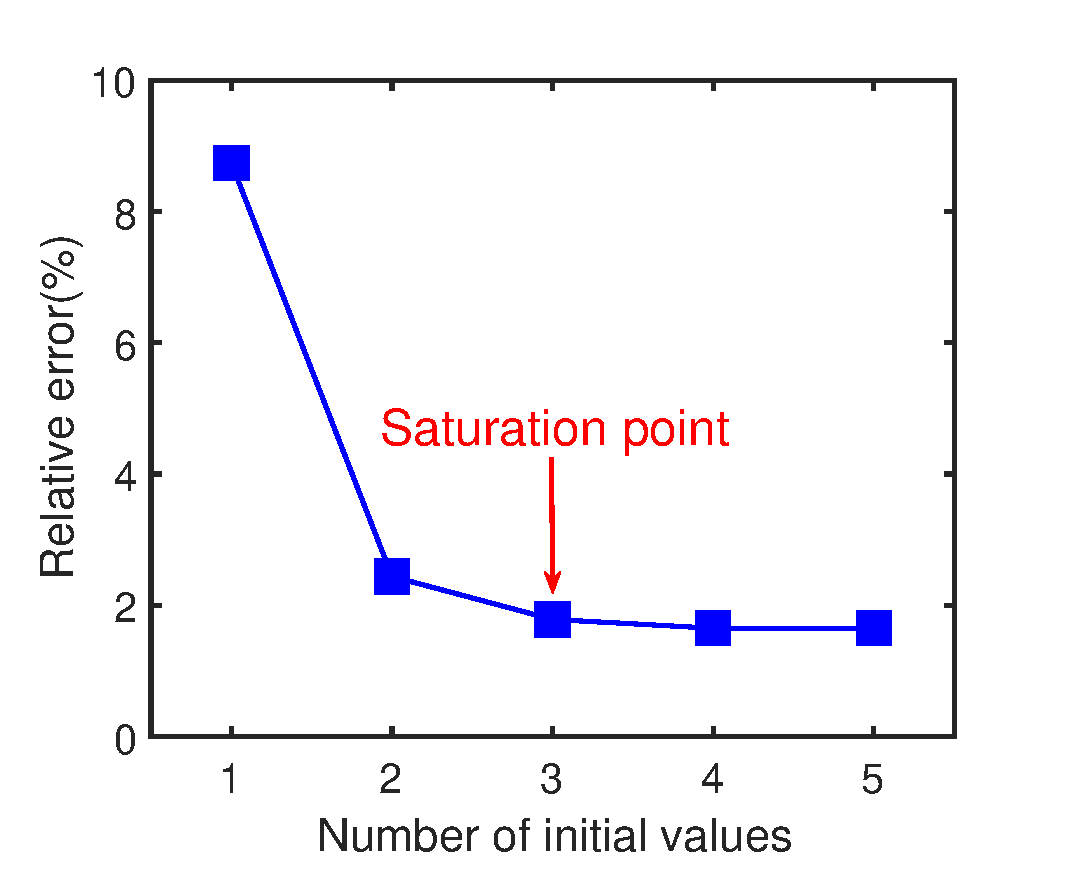
\includegraphics[scale=0.5]{fig_Niv.eps}
\par\end{centering}
\caption[Relative error for the total fit]{Relative error for the total fit, averaged over 1000 random spectra from the database, as a function of the number of initial values $N_{iv}$ for $\beta_\mathrm{BB}$ in the GG model.}
\label{fig:Niv}
\end{figure}
%%%%%%%%%%%%%%%%%%%%


\section{Parametrization results and discussion} \label{sec:parametrization_results_and_discussion}

\subsection{Statistical comparison}

To compare the fitting performance of the three models for the BB turbulence, the quality of the total fit was assessed for 10,000 spectra (about 3\% of the full database). Here, spectra with low SNR were not considered for the analysis even though the fitting results are good. The performance was evaluated by means of the minimal value of the cost function ($F_{cost,min}$) and the Bayesian information criterion ($BIC$). Assuming a Gaussian distribution of the measured spectrum around the fit, the BIC is given by \cite{Linden_2014_Bayesian}:%
%%%%%%%%%%%%%%%%%%%%
\begin{equation}
BIC = 2n \times ln(s) + K \times ln(n).
\label{eq:BIC}
\end{equation}
%%%%%%%%%%%%%%%%%%%%
\noindent Here, $n$ is the number of data points, $s$ is the standard deviation of the residuals, and $K$ is the number of parameters of the overall model. The BIC includes a penalty term for overly complex models, hence avoiding a preference for models that overfit the data. Figure \ref{fig:Error} shows the distribution of $F_{cost,min}$ and the BIC for all fits over the 10,000 spectra in the database. It can be seen that the generalized Gaussian and the Taylor model generally perform better than the Voigt (pseudo-Voigt) model. The generalized Gaussian model might still perform slightly better than the Taylor model.

%%%%%%%%%%%%%%%%%%%%
\begin{figure}[ht]
\begin{centering}
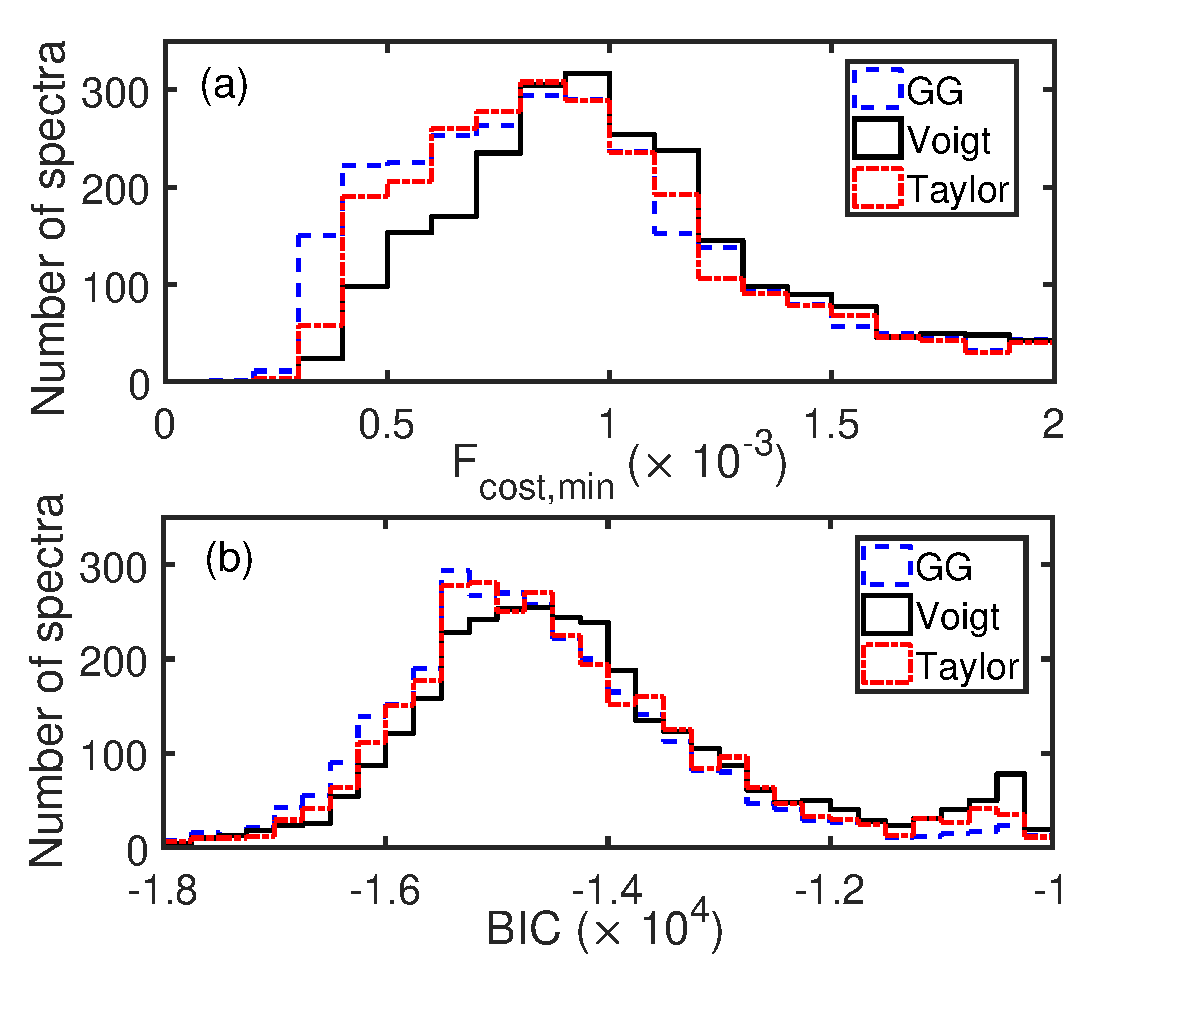
\includegraphics[scale=0.5]{fig_Error.eps}
\par\end{centering}
\caption[Comparison of the minimal value of the cost function and the Bayesian information criterion for the generalized Gaussian, the pseudo-Voigt and the Taylor model]{Comparison of (a) the minimal value of the cost function ($F_{cost,min}$) and (b) the Bayesian information criterion (BIC) for the generalized Gaussian (GG) function, the pseudo-Voigt function, and the Taylor function fitted to the BB turbulence component. The more a histogram contains low values of RSS and BIC, the better the performance of the corresponding model.}
\label{fig:Error}
\end{figure}
%%%%%%%%%%%%%%%%%%%%


\subsection{Representative spectral shapes} \label{sec:representative_spectral_shapes}

The statistical criteria studied above are only one aspect in assessing the fitted model. The fitting model should also conform to the criteria of flexibility, discrimination and robustness, and should be able to capture the salient physics reflected in the spectrum, especially the BB turbulence. In order to validate the superior performance of the generalized Gaussian and Taylor models, as suggested by the statistical analysis, some typical examples were investigated in detail. When the BB component has a Gaussian-like shape, the three models all show an equivalent, excellent fitting performance. In contrast, in case of a more difficult to fit Lorentzian or Laplacian (i.e. double exponential, or triangular on the logarithmic scale), the fitting results can be very different between the three models. This is shown on both the linear and logarithmic scales in figures \ref{fig:CmpHFS} and \ref{fig:CmpTRI}, which correspond to the approximate Lorentzian and Laplacian situation, respectively. On the linear scale, the fit is dominated by the low-frequency part ($f<25$ kHz), while on the logarithmic scale validation of the fitting performance should concentrate on the larger frequencies (up to 450 kHz).


For the Lorentzian shape in figure \ref{fig:CmpHFS}, visual inspection reveals a good fit by all three models, although the fit including the pseudo-Voigt model underpredicts the spectrum between 5 and 10 kHz (figure \ref{fig:CmpHFS} (c)) and around 100 kHz (figure \ref{fig:CmpHFS} (d)). This is reflected by its slightly worse RSS and BIC compared to the other two models. Another shortcoming of the pseudo-Voigt model is that it tends to fit also the noise, as can be seen in figure \ref{fig:CmpHFS} (d). Similar weaknesses of the pseudo-Voigt function can be seen in figure \ref{fig:CmpTRI}. For these reasons, we reject the Voigt function for fitting the BB turbulence.


%%%%%%%%%%%%%%%%%%%%
\begin{figure}[h]
\begin{centering}
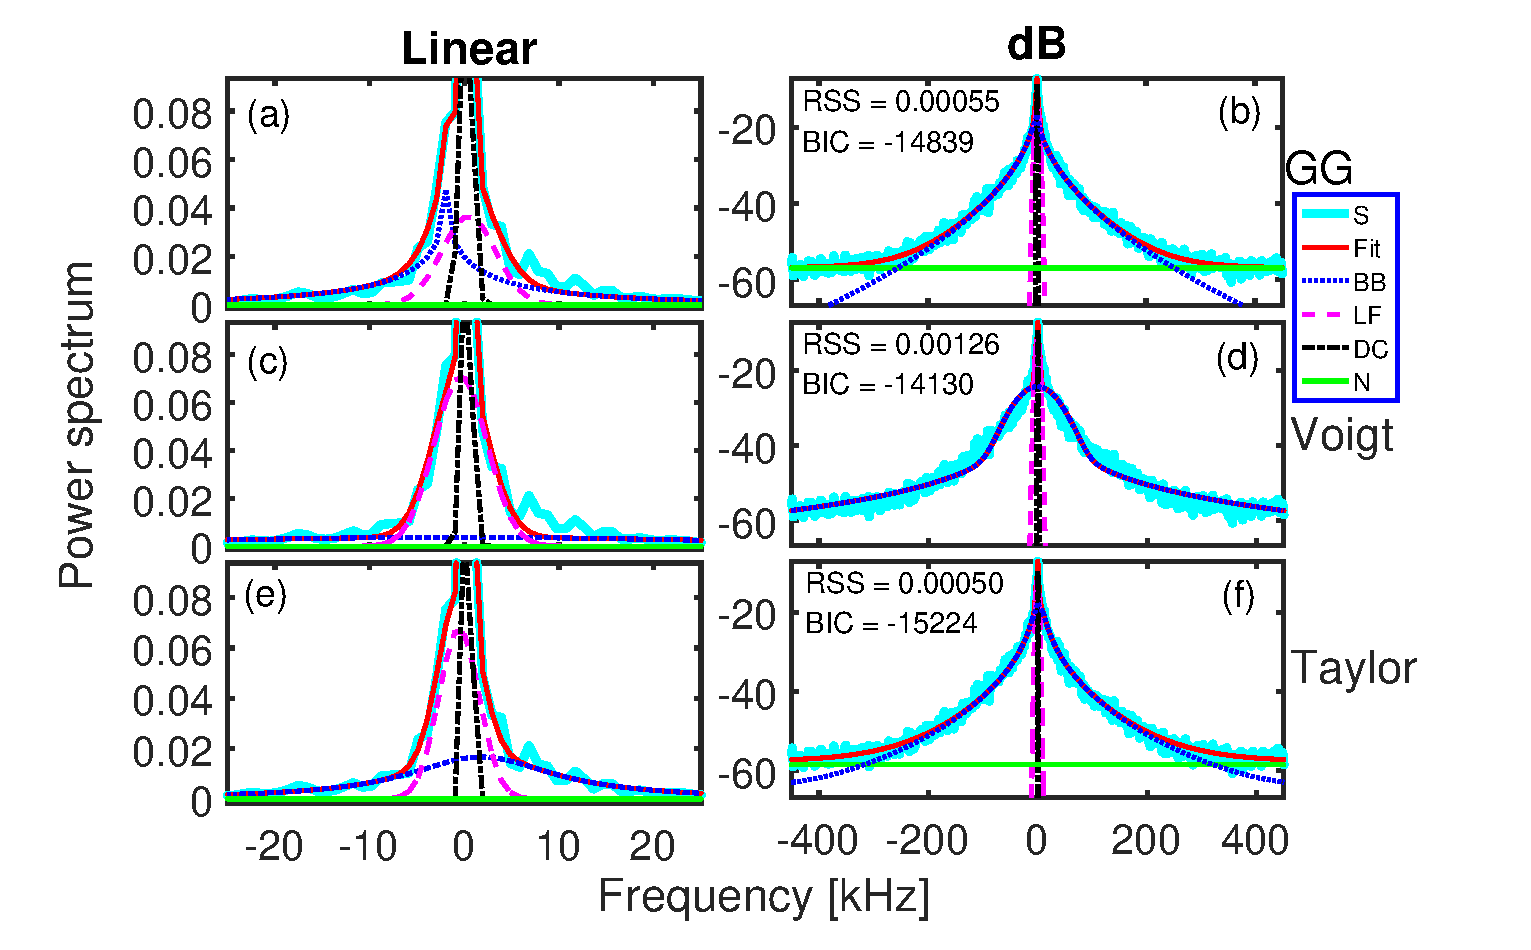
\includegraphics[scale=0.6]{fig_CmpHFS.eps}
\par\end{centering}
\caption[Fitting a Lorentzian spectrum]{Fit of a Lorentzian spectrum (S), with the individual components also displayed. The BB component was fitted by a generalized Gaussian (GG) function ((a) and (b)), the pseudo-Voigt function ((c) and (d)), and the Taylor function ((e) and (f)). The results are shown on the linear scale ((a), (c), (e)) and logarithmic (dB) scale ((b), (d), (f)). The residual sum of squares (RSS) and the Bayesian information criterion (BIC) at the optimal solution by each model are also displayed.}
\label{fig:CmpHFS}
\end{figure}
%%%%%%%%%%%%%%%%%%%%


When comparing the GG model with the Taylor model, it can be noted in figures \ref{fig:CmpHFS} and \ref{fig:CmpTRI} that the crucial difference is the peaked shape of the BB component in the GG model, whereas the Taylor model has a much smoother shape. From poloidal correlation in \cite{Kramer-Flecken_2015_NJP}, the BB component disappears when the LF component remains the same, meaning that the BB component does not have an intense low-frequency part. Hence, the fitting results in terms of the BB and LF components can be very different. In figures \ref{fig:CmpHFS} (a) and (e), the average frequencies w.r.t. the central frequency (0 KHz) for the BB and LF components have an opposite sign for the two models. Specifically, in figure \ref{fig:CmpHFS} (a), the peaked shape of the GG seems to fit the knee in the spectrum around 3 kHz, whereas this shape is not expected for the BB turbulence. In the case of the Lorentzian or Laplacian spectra, we observe that the estimated GG shape parameter often saturates at the lower bound $\beta_\mathrm{BB} = 0.5$, causing a peaked shape that tries to fit small-scale features in the spectrum. In turn, this may lead to overestimation of the BB contribution and instability of the BB standard deviation. Therefore, due to both excellent quantitative and qualitative performance, we choose the Taylor model as the optimal fit to the spectra. Nevertheless, the generalized Gaussian model is still useful since it allows a more direct study of the shape of the BB component through a single shape parameter, whereas the two shape parameters of the Taylor model ($\Delta_\mathrm{BB}$, $\tau_\mathrm{BB}$) are more difficult to interpret.


%%%%%%%%%%%%%%%%%%%%
\begin{figure}[ht]
\begin{centering}
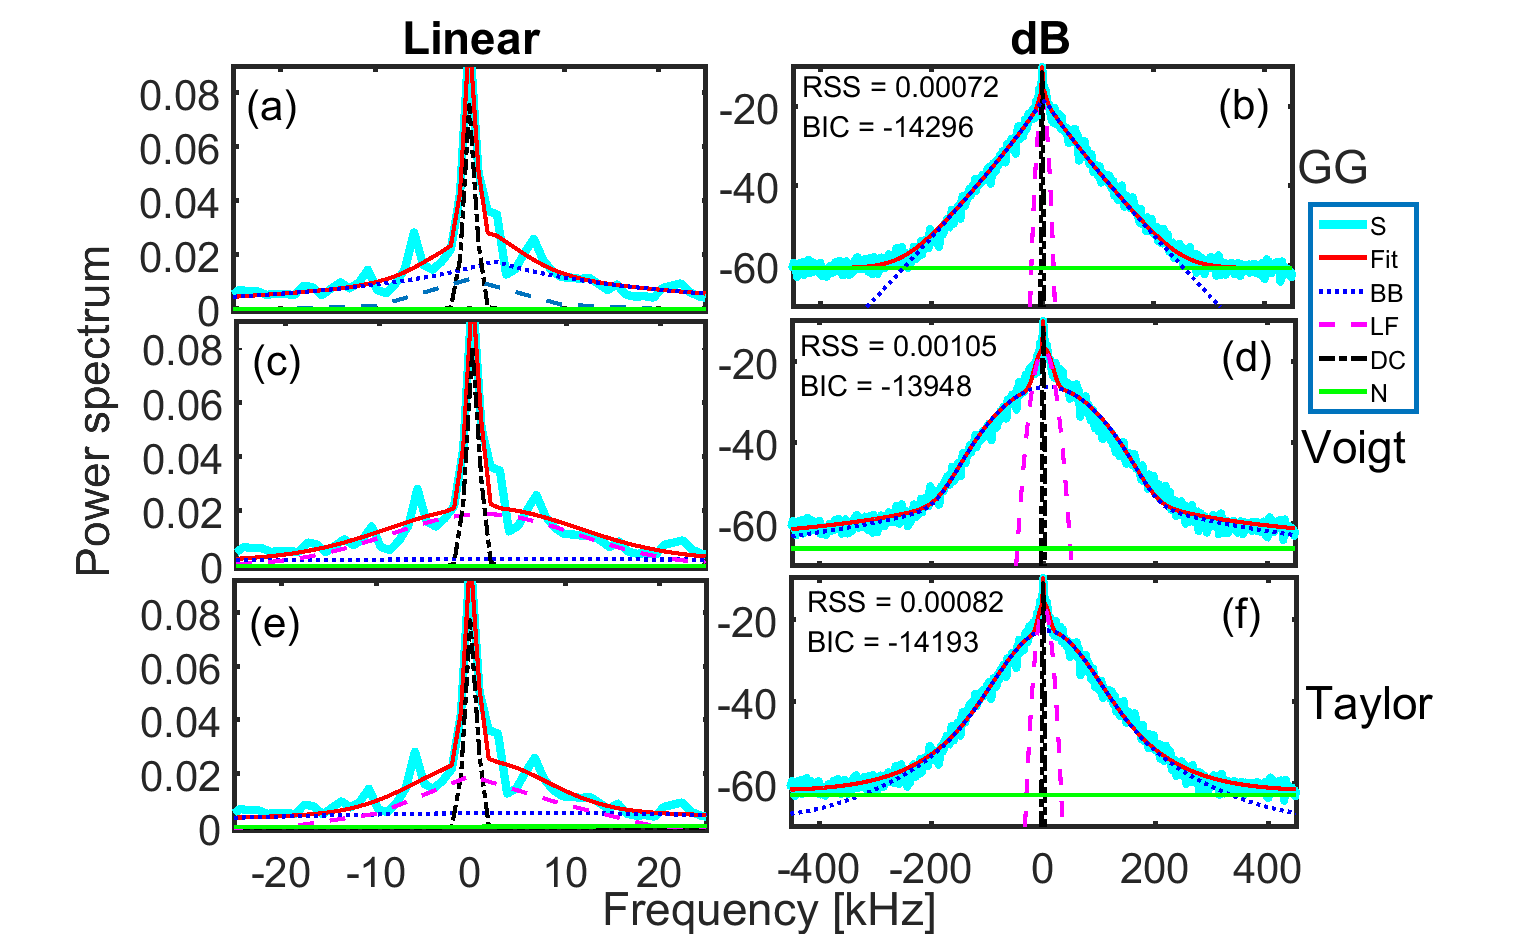
\includegraphics[scale=0.6]{fig_CmpTRI.eps}
\par\end{centering}
\caption[Fitting a Laplacian spectrum]{Same as figure \ref{fig:CmpHFS} for a Laplacian shape.}\label{fig:CmpTRI}
\end{figure}
%%%%%%%%%%%%%%%%%%%%


The reliability of fitting different components of spectra relies on the number of data for the corresponding components, i.e., more data points give better fit. Although the number of FFT has been chosen as 1024 to guarantee an accurate estimation of the low frequency part, there is still relatively limited data points for the LF and DC components, while the BB component has sufficient points for the fit. Therefore, the fitting parameters/results should be more stable in the BB fit than the LF and DC components. The parameters of the LF and DC components could become even less reliable when they saturate to the constrained maximum values. The situations occur especially when the integration or merging of the LF and BB component happens for some spectra shapes. 


\section{Turbulence database} \label{sec:turbulence_database}

The parametrization method was applied to core reflectometry measurements \cite{Sabot_2006_NF} from 6,000 Tore Supra discharges carried out between 2002 and 2011, and a large-scale turbulence database was built including 350,000 reflectometer acquisitions. The 6,000 discharges contain a large number of Ohmically heated plasmas, as well as plasmas with auxiliary heating: ICRH, LH and a limited number with ECRH \cite{Sun_2018_RSI}.

\subsection{Criteria of parameter filtering} \label{sec:Criteria_parameter}

An initial filtering of the database was deemed necessary, disregarding spectra with excessive noise or unwanted additional components, or in the presence of undesirable physical effects.

To quantify the noise level, the signal-to-noise ratio (SNR) is defined as the ratio between the amplitude of broadband component ($A_\mathrm{BB}$) and the noise ($\epsilon_N$): SNR $= A_\mathrm{BB}/\epsilon_N$. Spectra with too low SNR ($< 25$ dB) have been removed from the analysis. Such an example is shown in figure \ref{fig:spectra_removed} (a). Moreover, spectra with large Doppler effect (central shift $ \mu_\mathrm{BB} > 50$ kHz, e.g., figure \ref{fig:spectra_removed} (b)) have also been excluded, since in these cases the physical process and the probed wavenumber are different from the standard reflectometry measurement signals. Specifically, the standard measurement signals come from the perpendicular reflection of the probing waves at the cutoff positions, and therefore reflect the local fluctuations with very low wavenumber. Large Doppler shift results from backscattering at finite wavenumber. This backscattering could appear when the magnetic axis is not on the equatorial plane, causing the reflectometer line-of-sight to be off-normal w.r.t. the cutoff layer surface, or when the turbulent structures are tilted with respect to the poloidal direction. Toward the edge, the tilting of the reflective surface in the toroidal direction due to the magnetic field ripple can also lead to strong Doppler shift. In addition, before further analysis, only measurements performed during steady-state conditions have been studied. For example, the reflectometer acquisitions during the current or power ramp-up or ramp-down phase have been filtered out to avoid additional complexity.


The present study considers the complete radial extent of the plasmas, except for the edge region at the LFS, where the density fluctuation level ($\delta n/n$) reaches $\sim 10\%$ and nonlinear effects may complicate the analysis \cite{Sabot_2006_PPCF,Hornung_2013_PPCF}. Furthermore, spectra in the radial range at the LFS near the edge ($0.6 < \rho < 1$, with $\rho = r/a$ the normalized radius) are more prone to the large Doppler shift partly caused by the high ripple ($6\% $ at the plasma edge) of the magnetic field. Finally, this part of the plasma cannot be probed at low density due to the reflectometer frequency range. This condition occurs for low-density Ohmic discharges and most LH plasmas. For these reasons, the number of valid measurements is significantly reduced beyond $\rho > 0.6$, rendering estimation of trends unreliable in that region. In practice, the radial range was set to $-1 < \rho < 0.6$. Here, $\rho = 0$ denotes the plasma center and negative $\rho$ corresponds to the HFS.

%%%%%%%%%%%%%%%%%%%%
\begin{figure}[h]
\begin{centering}
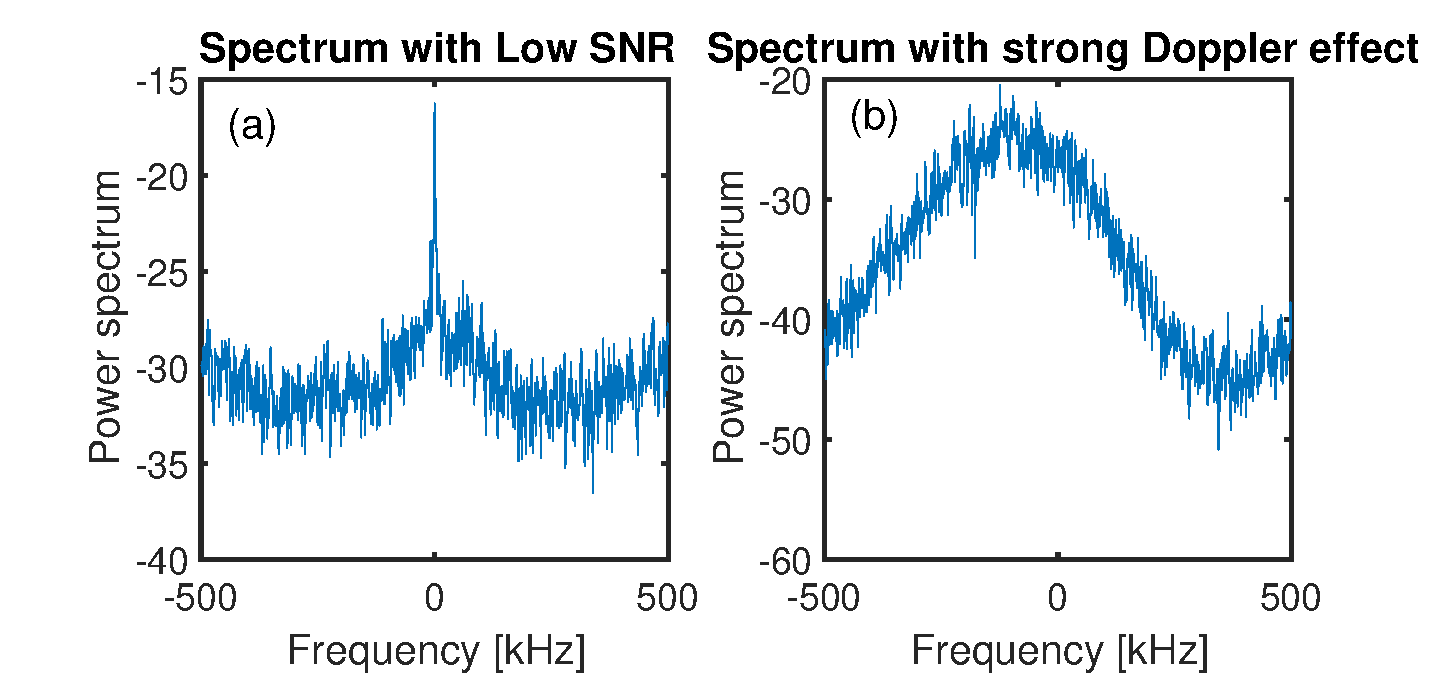
\includegraphics[scale=0.6]{fig_spectra_removed.eps}
\par\end{centering}
\caption{Representative spectrum with (a) low signal-to-noise ratio and (b) strong Doppler effect.}
\label{fig:spectra_removed}
\end{figure}
%%%%%%%%%%%%%%%%%%%%


\subsection{Parameters of the turbulence database} \label{sec:parameters_turbulence_database}

The database established in the framework of this PhD includes near 100 parameters that fall into four categories: the reflectometry diagnostic characteristics, the global operational parameters, the local plasma parameters and the spectrum characteristics.

The reflectometry diagnostic characteristics include acquisition parameters, as well as the probing frequencies ($100 \sim 155$ GHz) and the radius of the cutoff layer. The radius of the cutoff layer is recovered from the density profile obtained from an interferometry diagnostic \cite{Gil_2009_FST}, as the density profile from the reflectometer is not available during fluctuation measurements. The normalized radius $\rho$ of the cutoff layer ranges from $-1$ to $1$, covering the entire plasma region.

Other global and local plasma parameters are obtained or calculated from various diagnostic data available in the Tore Supra database. The global operational parameters include the on-axis toroidal magnetic field $B_{t,0}$, plasma current $I_{p}$, line-integrated electron density $n_l$, major radius $R$, minor radius $a$, plasma heating power, elongation, edge safety factor ($q_{\psi}$) and the heating power for different scenarios ($P_\mathrm{Ohmic}$, $P_\mathrm{ICRH}$, $P_\mathrm{LH}$, $P_\mathrm{ECRH}$), etc. The local plasma parameters include the electron density $n_e(r)$ from interferometry measurements, the electron temperature $T_e(r)$ from ECE measurements, as well as the gradients of density, temperature and refractive index at the cutoff obtained from various density, temperature and magnetic diagnostics.



The spectrum characteristics initially include the 11 spectrum decomposition parameters. From these parameters, we derive the following additional quantities to systematically investigate general trends of the turbulence properties across the database. First, the BB contribution ($E_\mathrm{BB}$) of the frequency spectrum in each spectrum is calculated by integrating the BB component, i.e. the broadband contribution in the spectrum divided by the total power of the spectrum:%
%%%%%%%%%%%%%%%%%%%%
\begin{equation}
  E_\mathrm{BB} = \frac{\int_{f_{min}}^{f_{max}} C_\mathrm{BB}(f)\,\mathrm{d} f}{\mathrm{Total\ spectrum\ power}}.
  \label{eq:EBB}
\end{equation}
%%%%%%%%%%%%%%%%%%%%
\noindent This is shown by the green shaded area in Figure \ref{fig:FitSpecBB} for three typical BB spectral shapes---(approximately) (a) Gaussian, (b) double exponential (Laplacian) and (c) Lorentzian (Cauchy) using the Taylor model. The contribution of the other components were obtained by a similar definition, so $E_\mathrm{DC} + E_\mathrm{LF} + E_\mathrm{BB} + E_\mathrm{Noise} \approx 1$ for a valid fitting after filtering. Furthermore, when the contribution of the noise is negligible ($E_\mathrm{Noise} \sim 0$), we should have $E_\mathrm{BB} \approx 1 - E_\mathrm{DC+LF}$, where $E_\mathrm{DC+LF} = E_\mathrm{DC} + E_\mathrm{LF}$ is the total energy contribution of the low-frequency parts in the spectra. From \eqref{eq:EBB}, $E_\mathrm{BB}$ ranges between 0 and 1. This means that all the energy of the spectrum is in the BB component when $E_\mathrm{BB} = 1$ and in the low-frequency parts when $E_\mathrm{BB} = 0$. In other words, $E_\mathrm{BB}$ reflects the relative intensity of the energy distribution between the BB component and the low-frequency parts. Since the fitting parameters are more stable for the BB component, $E_\mathrm{BB}$ has a more accurate estimation of the energy contribution than $E_\mathrm{LF}$.


%%%%%%%%%%%%%%%%%%%%
\begin{figure}[h]
\begin{centering}
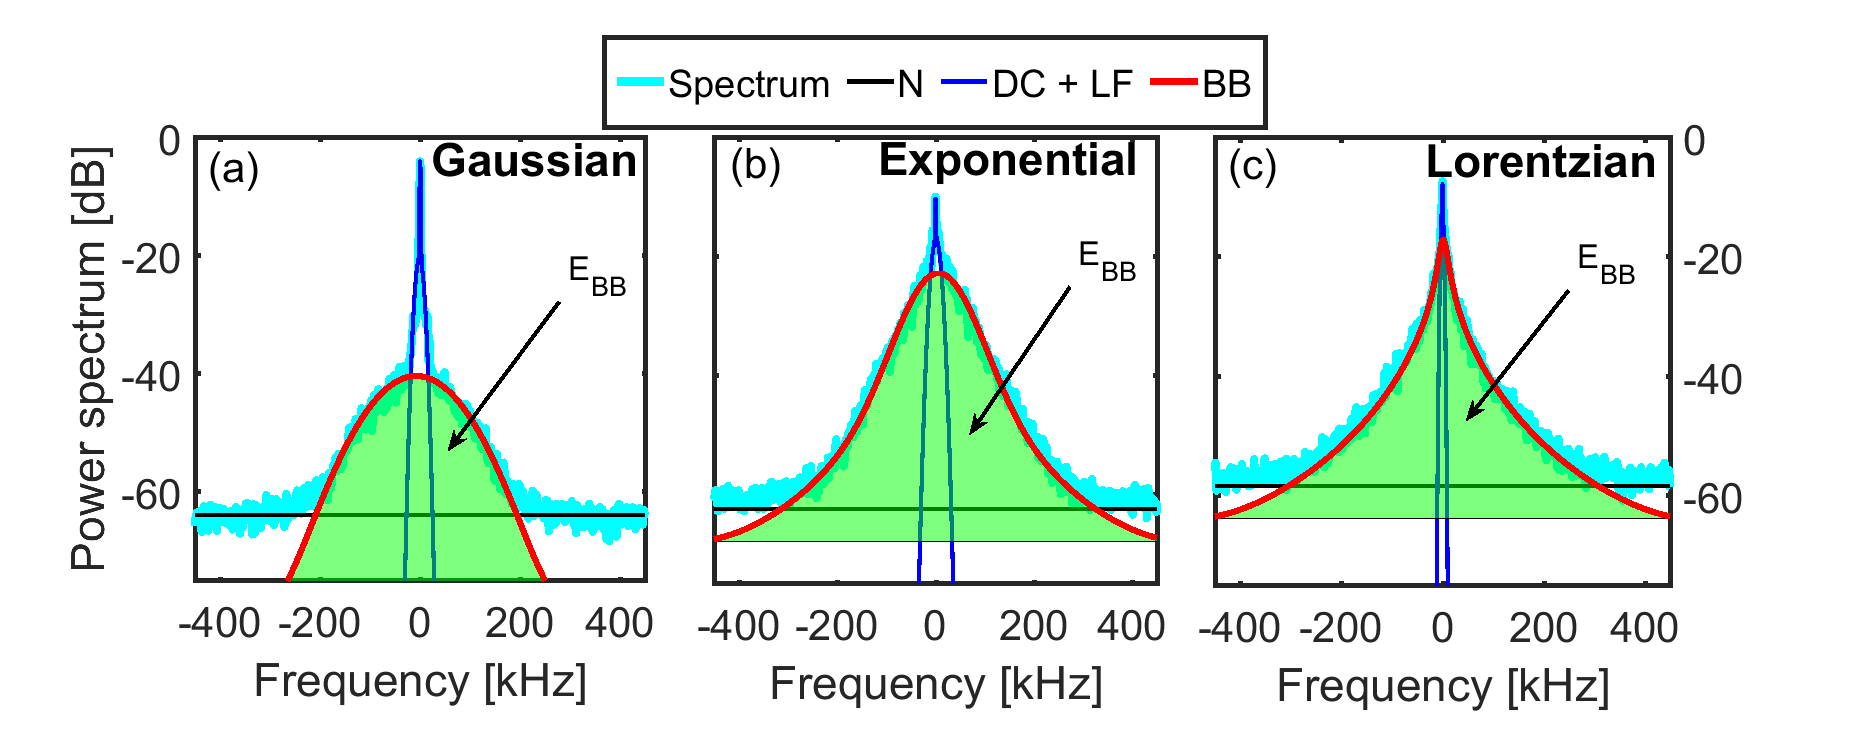
\includegraphics[scale=0.5]{fig_FitSpecBB.eps}
\par\end{centering}
\caption{Components of typical reflectometry spectra with varying shapes: approximately (a) Gaussian, (b) double exponential (triangular on the logarithmic scale) and (c) Lorentzian. The DC and LF components were fitted by two Gaussian functions, the noise level (N) by a constant and the BB component by the FFT of the Taylor function. The green shaded area represents the integrated BB contribution, denoted by $E_\mathrm{BB}$.}
\label{fig:FitSpecBB}
\end{figure}
%%%%%%%%%%%%%%%%%%%%


Additional fluctuation properties can be obtained from the parametrization, e.g. the standard deviation, i.e. the square root of the second central moment of the BB and LF component, which we refer to as the \emph{BB width} ($W_\mathrm{BB}$) and the LF width ($W_\mathrm{LF}$). The parameters of spectral energy and width come from the Taylor model, due to its superior performance compared to the other models. In addition, the exponent ($\beta_\mathrm{BB}$) in the generalized Gaussian function provides a convenient measure for the shape of the BB component, which is strongly related to the kurtosis of the distribution.

The structure of the database is listed in table \ref{table:turbulence_database}, by means of a number of commonly used entries or parameters. All the plasma parameters corresponding to each spectrum (each index in the table) are calculated as the average value during the acquisition time window of each reflectometry fluctuation measurement (typically 10 ms).


%%%%%%%%%%%%%%%%%%%%
\begin{table}[h]
  \centering

  \begin{tabular}{|c|c|c|c|c|c|c|c|c|c|c|}
    \hline
    % after \\: \hline or \cline{col1-col2} \cline{col3-col4} ...
    Index  & $\rho$ & $B_{t,0}$  & $I_p$ & $q_{\psi}$ & $n_e$ & $T_e$ & $E_\mathrm{BB}$ & $W_\mathrm{BB}$ & $\beta_\mathrm{BB}$ & $\dots$ \\
    \hline
    1      & $0.65$ & $3.86$   & $1.0$   & $3.64$  & 3.5  & 2  & 0.1 & 50 & $\dots$ & $\dots$ \\
    2      & $0.54$ & $3.46$   & $1.0$   & $3.63$  & 4.0  & 3  & 0.5 & 100 & $\dots$ & $\dots$ \\
    $\dots$  & $\dots$  & $\dots$    & $\dots$   & $\dots$   & $\dots$ & $\dots$ & $\dots$ & $\dots$  & $\dots$ & $\dots$ \\
    \hline
  \end{tabular}

  \caption{Structure of the turbulence database built from the Tore Supra database. The index in the first column of the table indicates the serial number of the spectra. The units of $B_{t,0}$, $I_p$, $n_e$, $T_e$ and $W_\mathrm{BB}$ are T, MA, $10^{19}m^{-3}$ and kHz, respectively.}
  \label{table:turbulence_database}

\end{table}
%%%%%%%%%%%%%%%%%%%%
